\chapter{Конструкторская часть}

\section{Схемы алгоритмов}

На рисунках 2.1 -- 2.4 представлены схемы алгоритмов 

\begin{figure}[h!]
	\centering
	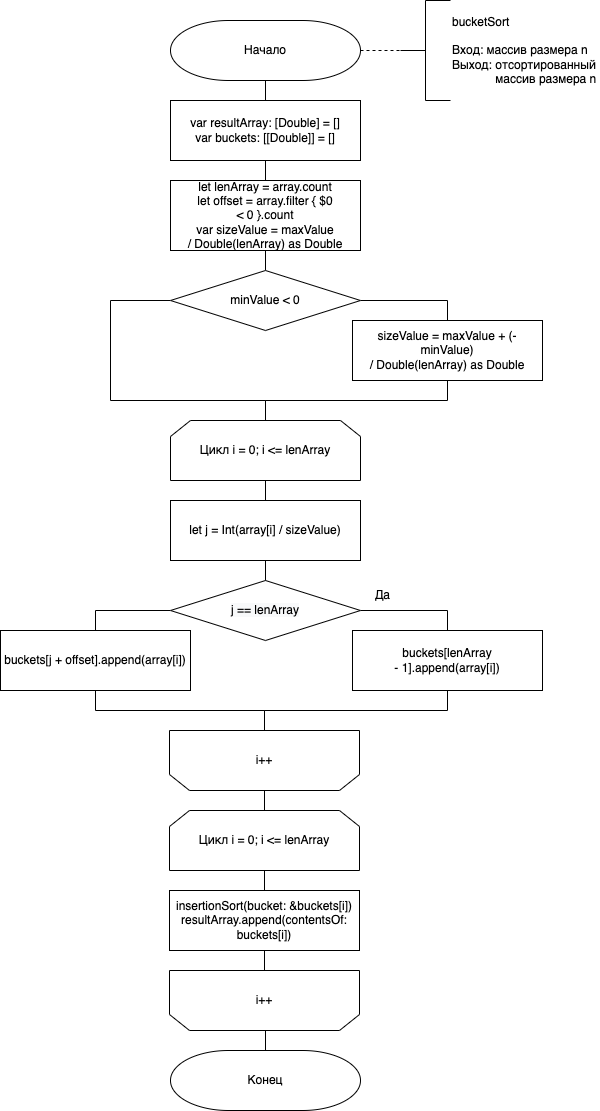
\includegraphics[width=0.8\linewidth]{img/Bucket.png}
	\caption{Схема алгоритма блочной сортировки}
	\label{fig:mpr}
\end{figure}

\begin{figure}[h!]
	\centering
	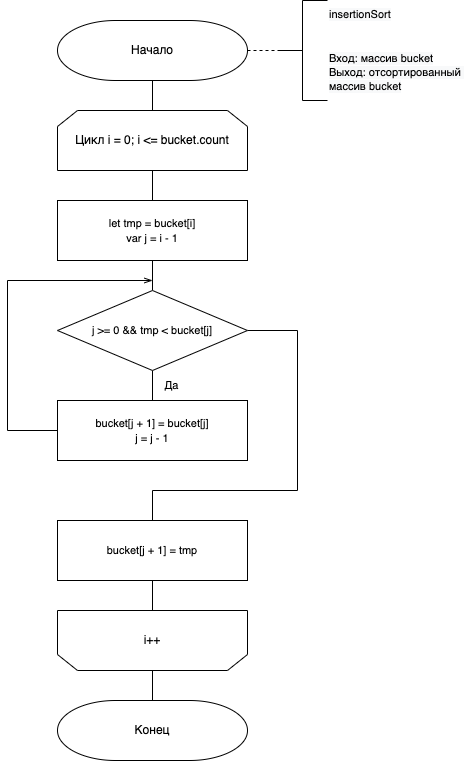
\includegraphics[scale=0.8]{img/Insertion.png}
	\caption{Схема алгоритма сортировки перемешиванием}
	\label{fig:mpr}
\end{figure}

\begin{figure}[h!]
	\centering
	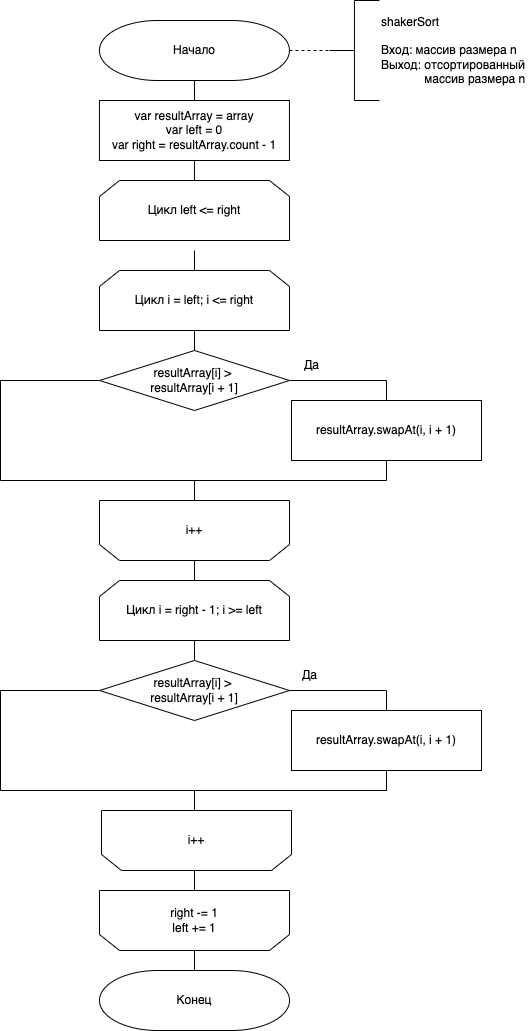
\includegraphics[scale=0.65]{img/Shaker.png}
	\caption{Схема алгоритма сортировки перемешиванием}
	\label{fig:mpr}
\end{figure}

\begin{figure}[h!]
	\centering
	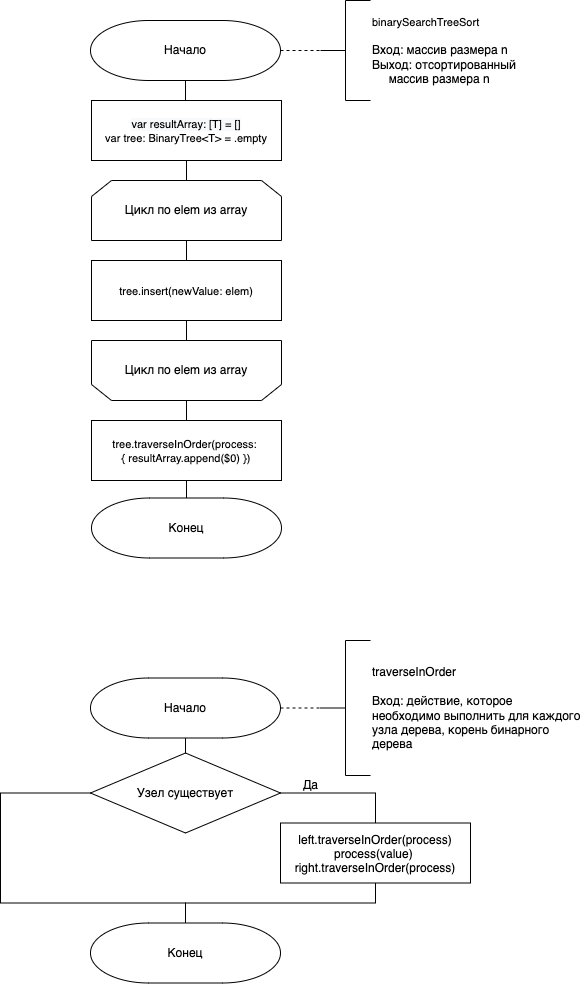
\includegraphics[scale=0.65]{img/BinaryTree.png}
	\caption{Схема алгоритма сортировки бинарным деревом}
	\label{fig:mpr}
\end{figure}

\section{Модель вычислений}

Для последующего вычисления трудоемкости введём модель вычислений.

\begin{enumerate}
	\item Операции из списка (\ref{for:opers}) имеют трудоемкость 1.
	\begin{equation}
	\label{for:opers}
	+, -, /, \%, ==, !=, <, >, <=, >=, [], ++, {-}-
	\end{equation}
	\item Трудоемкость оператора выбора if условие then A else B рассчитывается по формуле (\ref{for:if}).
	\begin{equation}
	\label{for:if}
	f_{if} = f_{\text{условия}} +
	\begin{cases}
	f_A, & \text{если условие выполняется,}\\
	f_B, & \text{иначе.}
	\end{cases}
	\end{equation}
	\item Трудоемкость цикла рассчитывается по формуле (\ref{for:for}).
	\begin{equation}
	\label{for:for}
	f_{for} = f_{\text{инициализации}} + f_{\text{сравнения}} + N(f_{\text{тела}} + f_{\text{инкремента}} + f_{\text{сравнения}})
	\end{equation}
	\item Трудоемкость вызова функции равна 0.
\end{enumerate}

\section{Трудоёмкость алгоритмов}

\subsection{Алгоритм блочной сортировки}

\begin{itemize}
	\item Трудоёмкость каждого из двух циклов $while$, которая вычисляется по формуле (\ref{for:bubble_outer1}).
	\begin{equation}
		\label{for:bubble_outer1}
		f_{outer1} = 2 + 2 \cdot (N - 1).
	\end{equation}
	\item Суммарная трудоёмкость первого цикла, количество итераций которых меняется в промежутке $[1..N-1]$, которая вычисляется по формуле (\ref{for:bubble_inner1}).
	\begin{equation}
		\label{for:bubble_inner1}
		f_{inner1} = 2(N - 1) + \frac{2 \cdot (N - 1)}{2} \cdot (4 + f_{if1}).
	\end{equation}
	\item Трудоёмкость условия в первом цикле, которая равна (\ref{for:bubble_if1}).
	\begin{equation}
		\label{for:bubble_if1}
		f_{if1} = 4.
	\end{equation}
	\item Суммарная трудоёмкость второго цикла, количество итераций которых меняется в промежутке $[1..N-1]$, которая вычисляется по формуле (\ref{for:bubble_inner1}).
	\begin{equation}
		\label{for:bubble_inner1}
		f_{inner} = 2 \cdot (N - 1) + f_{ins1}.
	\end{equation}
	\item Трудоёмкость внешнего цикла сортировки вставками, которая вычисляется по формуле(\ref{for:ins1}).
	\begin{equation}
		\label{for:ins1}
		f_{ins} = 3 \cdot (N - 1) + f_{inner1}.
	\end{equation}
\end{itemize}

Трудоёмкость в \textbf{лучшем} случае (\ref{for:bbest}).
\begin{equation}
	\label{for:bbest}
	f_{best} = 4 + \frac{3}{2} N + f_{ins} \approx K= O(N + K).
\end{equation}

Трудоёмкость в \textbf{худшем} случае (\ref{for:bworst}).
\begin{equation}
	\label{for:bworst}
	f_{worst} = 4 + \frac{3}{2} N + f_{ins} \approx K= O(N + K).
\end{equation}


\subsection{Алгоритм сортировки вставками}

Используется в блочной сортировке. 

\begin{itemize}
	\item Трудоёмкость сравнения и инкремента внешнего цикла в промежутке $[1..N-1]$, которая вычисляется по формуле (\ref{for:isort_outer}).
	\begin{equation}
	\label{for:isort_outer}
	f_{i} = 2 + 2(N - 1).
	\end{equation}
	\item Суммарная трудоёмкость внутренних циклов, количество итераций которых меняется в промежутке $[1..N-1]$, которая вычисляется по формуле (\ref{for:isort_inner}).
	\begin{equation}
	\label{for:isort_inner}
	f_{if} = 4 + \begin{cases}
		0, & \text{в лучшем случае}\\
		3(N - 1) + \frac{N \cdot (N - 1)}{2} \cdot (3 + f_{if}), & \text{в худшем случае}\\
	\end{cases}
	\end{equation}

	\item Трудоёмкость условия во внутреннем цикле, которая вычисляется по формуле (\ref{for:isort_if}).
	\begin{equation}
	\label{for:isort_if}
	f_{if} = 4 + \begin{cases}
	0, & \text{в лучшем случае}\\
	9, & \text{в худшем случае}\\
	\end{cases}
	\end{equation}
\end{itemize}

Трудоёмкость в \textbf{лучшем} случае (\ref{for:isort_best}):
\begin{equation}
\label{for:isort_best}
f_{best} = 13N - 10 \approx 13N = O(N).
\end{equation}

Трудоёмкость в \textbf{худшем} случае (\ref{for:isort_worst}):
\begin{equation}
\label{for:isort_worst}
f_{worst} = 4.5N^2 + 10N - 13 \approx 4N^2 = O(N^{2}).
\end{equation}

\subsection{Алгоритм сортировки перемешиванием}

\begin{itemize}
	\item Трудоёмкость сравнения внешнего цикла $while$, которая вычисляется по формуле (\ref{for:bubble_outer}).
	\begin{equation}
		\label{for:bubble_outer}
		f_{outer} = 1 + 2 \cdot (N - 1).
	\end{equation}
	\item Суммарная трудоёмкость внутренних циклов, количество итераций которых меняется в промежутке $[1..N-1]$, которая вычисляется по формуле (\ref{for:bubble_inner}).
	\begin{equation}
		\label{for:bubble_inner}
		f_{inner} = 5(N - 1) + \frac{2 \cdot (N - 1)}{2} \cdot (3 + f_{if}).
	\end{equation}
	\item Трудоёмкость условия во внутреннем цикле, которая вычисляется по формуле (\ref{for:bubble_if}).
	\begin{equation}
		\label{for:bubble_if}
		f_{if} = 4 + \begin{cases}
			0, & \text{л.с.}\\
			9, & \text{х.с.}\\
		\end{cases}
	\end{equation}
\end{itemize}

Трудоёмкость в \textbf{лучшем} случае (\ref{for:bubble_best}):
\begin{equation}
	\label{for:bubble_best}
	f_{best} = -3 + \frac{3}{2} N + \approx \frac{3}{2} N = O(N).
\end{equation}

Трудоёмкость в \textbf{худшем} случае (\ref{for:bubble_worst}):
\begin{equation}
	\label{for:bubble_worst}
	f_{worst} = -3 - 8N + 8N^2 \approx 8N^2 = O(N^2).
\end{equation}

\subsection{Алгоритм сортировки бинарным деревом}
Процедура добавления объекта в бинарное дерево имеет среднюю алгоритмическую сложность порядка $O(log(N))$. Соответственно, для N объектов сложность будет составлять $O(N log(N))$ \cite{otree}.

\section{Вывод}
На основе теоретических данных, полученных из аналитического раздела, были построены схемы всех алгоритмов сортировки массивов, а также описана модель вычислений и, исходя из нее, оценена трудоемкость для каждого алгоритма. 
